% src/slides/source/final/core/02_problem.tex

\begin{frame}{Problem}
  \SlideBody{\begin{VisualCanvas}
    \node[final statement,text width=14.4cm,
      font=\sffamily\fontsize{16}{20}\selectfont] at (7.4,5.28)
      {Can a Holistic Early-Fusion Model Be Compressed\\
      While Preserving Detection Accuracy?};
    \begin{scope}[yshift=-0.20cm,overlay]
      \node[inner sep=0pt] at (7.4,2.70)
        {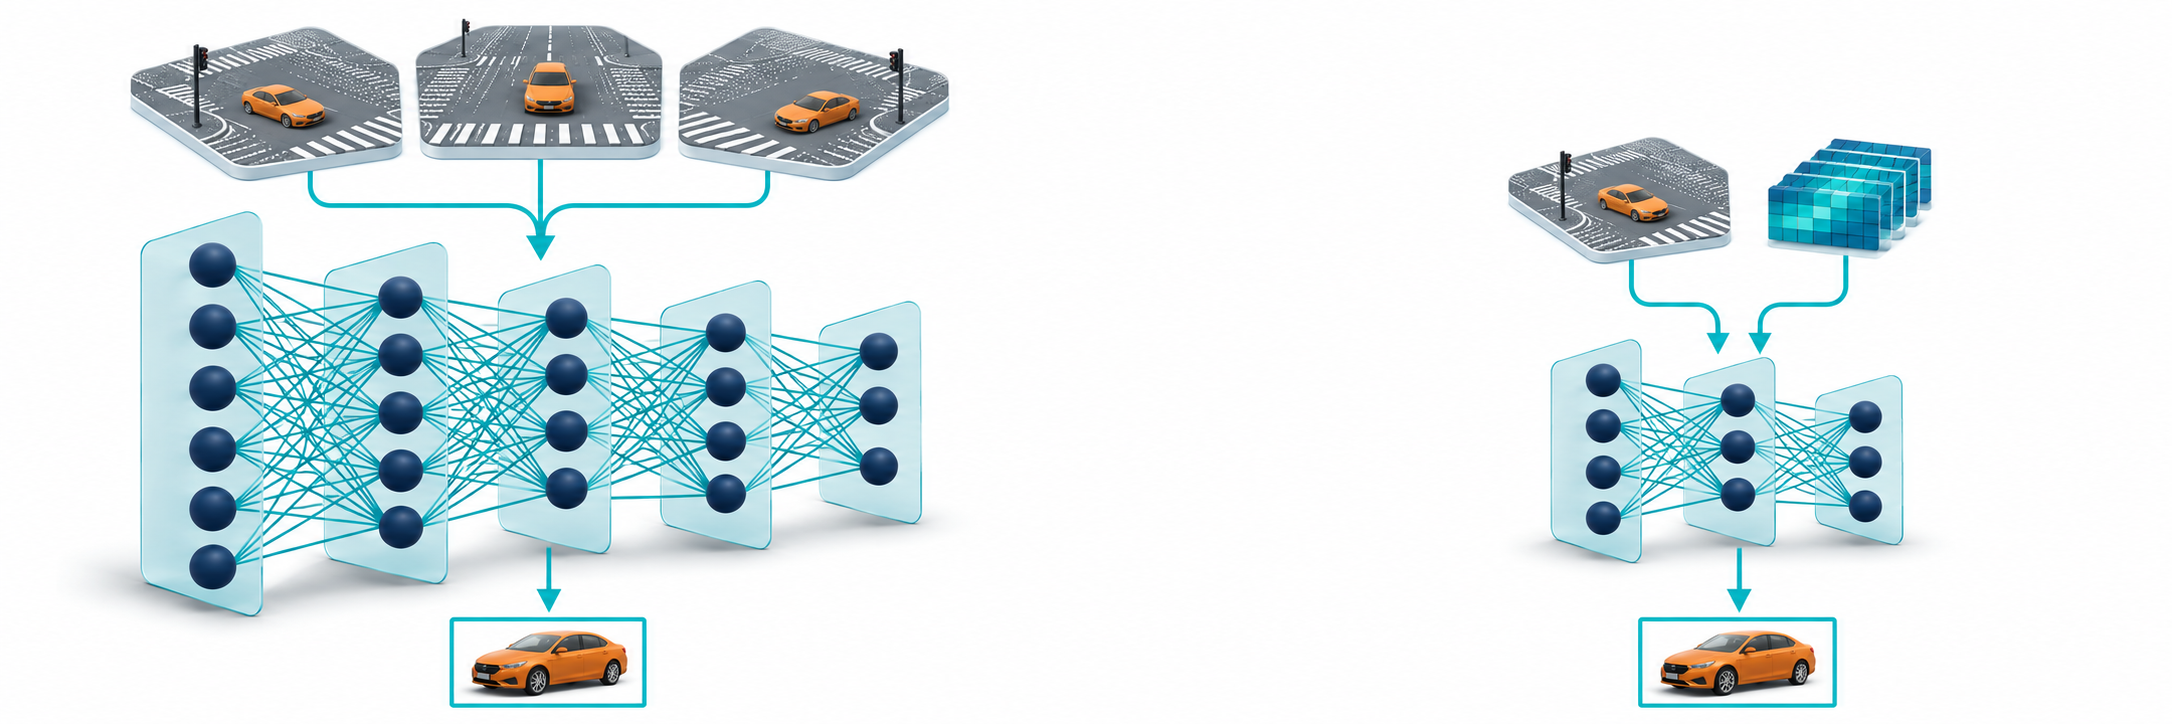
\includegraphics[width=11.7cm]{assets/illustrations/problem/problem-model-distillation-imagegen-v4.png}};
      \node[final heading] at (4.5,0.55) {Teacher};
      \node[final heading] at (11.0,0.55) {Student};
      \node[visual small,anchor=center] at (4.5,0.14) {Holistic View};
      \node[visual small,anchor=center] at (11.0,0.14) {Local + Shared Features};
      \draw[visual arrow,dashed] (6.90,2.70) --
        node[above,align=center,text=MoverNavy,font=\fontsize{9}{11}\selectfont]
          {Distillation\\Training Only} (9.90,2.70);
    \end{scope}
  \end{VisualCanvas}}
  \SlideSource{Source: AI generated illustrations.}
\end{frame}
